% Ubah judul dan label berikut sesuai dengan yang diinginkan.
\section{Results and Analysis}
\label{sec:resultnanalysis}

\par Bab ini akan membahas hasil dan analisa dari desain sistem yang sudah dibuat dan implementasinya. Pengujian terhadap hasil dibagi menjadi beberapa bagian.

\subsection{Pengujian Performa antar \emph{Weight}}
\label{subsec:modeltest}
% Ubah paragraf-paragraf pada bagian ini sesuai dengan yang diinginkan.

% \par The YOLOv5 repository provides several checkpoints or weights that result from training the YOLOv5 model from the COCO dataset used as a pre-trained model. The expectation of using this pre-trained model is that the resulting weight will perform better than doing training without any pretrained model. This COCO dataset has 80 different classes. However, as mentioned in \ref{subsec:dataset_labeling}, this research, only requires 2 classes, namely "no\_helmet" and "with\_helmet".

\par Repositori YOLOv5 menyediakan beberapa \emph{checkpoint} atau \emph{weight} yang merupakan hasil training model YOLOv5 dari dataset COCO yang dimanfaatkan sebagai \emph{pretrained model}. Ekspektasi penggunaan pretrained model ini yaitu bobot yang dihasilkan akan memiliki performa yang lebih tinggi daripada melakukan training tanpa pretrained model sama sekali. \emph{COCO Dataset} ini memiliki 80 \emph{class} berbeda. Seperti disebutkan pada \ref{subsec:dataset_labeling} yaitu untuk keperluan penelitian ini hanya memerlukan 2 kelas yaitu "no\textunderscore helmet" dan "with\textunderscore helmet".

% \par Some of the pre-trained models provided from the YOLOv5 repository are YOLOv5n, YOLOV5s, YOLOv5m, YOLOv5l, YOLOv5l, and YOLOv5x. In addition to these pre-trained models, there is also a version for the 1280 image size, namely the YOLOv5n6 to YOLOv5l6 series. In this study, only the YOLOv5n to YOLOv5l variations are used because the YOLOv5x variation and the 6 series version for 1280 image sizes take longer. The differences in the pre-trained weights stem from the initial configuration of training on the COCO dataset using YOLOv5, especially the "depth\_multiple" and "width\_multiple" parameters.

\par Beberapa \emph{pretrained model} yang disedikana dari repositori YOLOv5 yaitu YOLOv5n, YOLOV5s, YOLOv5m, YOLOv5l,YOLOv5l, dan YOLOv5x. Selain beberapa model pretrained tersebut juga ada versi untuk ukuran gammbar 1280 yaitu seri YOLOv5n6 hingga YOLOv5l6. Pada penelitian ini hanya menggunakan variasi YOLOv5n hingga YOLOv5l karena variasi YOLOv5x dan versi seri 6 untuk ukuran gambar 1280 membutuhkan waktu yang lebih lama. Perbedaan - perbedaan yang ada pada bobot - bobot pretrained tersebut berasal dari konfigurasi awal dari training pada dataset COCO yang menggunakan YOLOv5, terutama pada paramter "depth\textunderscore multiple" dan "width\textunderscore multiple".

% \par The validation process of the training results is carried out using the Safety Helmet Detection dataset, whose distribution is described in the \ref{subsec:dataset_preprocessing} section, which consists of 1200 images with the "no\_helmet" class totalling 1322 labels and the "with\_helmet" class totalling 4294 labels.

\par Proses validasi hasil training dilakukan menggunakan dataset Deteksi Helm Keselamatan Kerja yang pembagiannya dijelaskan pada bagian \ref{subsec:dataset_preprocessing} yang berjumlah 1200 gambar dengan kelas "no\textunderscore helmet" berjumlah 1322 label dan kelas "with\textunderscore helmet" berjumlah 4294 label.

% \par In this section, we will compare the performance of each weight generated with the pre-trained model and those without the pre-trained model. This test was carried out using resources from Google Colab. The Google Colab resource specifications used when validating for weights that have been {trained} can be seen in Table~\ref{tb:spekgoogleclab}.

\par Pada bagian ini akan dipaparkan dan dibandingkan performa antara tiap bobot yang dihasilkan dengan model pretrained dan yang tidak menggunakan pretrained model. Pengujian ini dilakukan menggunakan \emph{resource} dari Google Colab. Spesifikasi \emph{resource} Google Colab yang digunakan saat melakukan validasi untuk bobot yang sudah di-\emph{train} dapat dilihat pada Tabel~\ref{tb:spekgoogleclab}.

\begin{table}
  \centering
  \caption{Spesifikasi \emph{Resource} Google Colab Untuk Validasi \emph{Weight}}
  \label{tb:spekgoogleclab}
  \begin{tabular}{|l|l|} 
  \hline
  Type    & Detail                      \\ 
  \hline
  Python  & Python-3.7.13                   \\
  PyTorch & torch-1.11.0+cu113              \\
  GPU     & Tesla P100-PCIE-16GB, 16281MiB  \\
  \hline
  \end{tabular}
\end{table}

\begin{table*}
  \centering
  \caption{Pretrained Model Peformance Test Result}
  \label{tb:pretrainbenchmarktest}
  \begin{tabular}{|l|l|l|l|l|l|l||} 
    \hline
    Weight Name                          & class        & precision & recall & mAP   & mAP .5:.95 & inference time (ms)    \\ 
    \hline
    \multirow{3}{*}{hedec\_pretrain\_N} & all          & 0.925     & 0.871  & 0.922 & 0.557      & \multirow{3}{*}{1.9}   \\
                                        & no\_helmet   & 0.924     & 0.867  & 0.916 & 0.552      &                        \\
                                        & with\_helmet & 0.926     & 0.875  & 0.929 & 0.562      &                        \\ 
    \hline
    \multirow{3}{*}{hedec\_pretrain\_S} & all          & 0.929     & 0.878  & 0.929 & 0.568      & \multirow{3}{*}{4}     \\
                                        & no\_helmet   & 0.925     & 0.857  & 0.918 & 0.561      &                        \\
                                        & with\_helmet & 0.932     & 0.9    & 0.941 & 0.575      &                        \\ 
    \hline
    \multirow{3}{*}{hedec\_pretrain\_M} & all          & 0.923     & 0.891  & 0.933 & 0.57       & \multirow{3}{*}{8.7}   \\
                                        & no\_helmet   & 0.919     & 0.883  & 0.923 & 0.561      &                        \\
                                        & with\_helmet & 0.928     & 0.898  & 0.943 & 0.58       &                        \\ 
    \hline
    \multirow{3}{*}{hedec\_pretrain\_L} & all          & 0.919     & 0.867  & 0.919 & 0.579      & \multirow{3}{*}{14}    \\
                                        & no\_helmet   & 0.904     & 0.846  & 0.899 & 0.565      &                        \\
                                        & with\_helmet & 0.934     & 0.887  & 0.939 & 0.593      &                        \\ 
    \hline
  \end{tabular}
\end{table*}

% \par Based on the validation results presented, there is no significant difference in precision, recall, mAP@.5 in either the "with\_helmet" or "no\_helmet" classes, as shown in Figure~\ref{tb:pretrainbenchmarktest}. The precision value is above 0.9, with the highest value being the "hedec\_pretrain\_S" variant. The recall is also not too different between the weights where everything is above the number 0.8, with the highest value being the "hedec\_pretrain\_M" variant.

\par Berdasarkan hasil validasi yang dipaparkan, tidak ada perbedaan signifikan dari \emph{precision, recall, mAP} 
baik pada kelas "with\_helmet" ataupun "no\_helmet" seperti yang ditunjukan pada Tabel~\ref{tb:pretrainbenchmarktest}.
Untuk nilai \emph{precision} berada di atas 0.9 dengan nilai tertinggi oleh varian "hedec\_pretrain\_S" . Untuk \emph{recall}
juga tidak terlalu berbeda diantara bobot dimana semuanya berada diatas angka 0.8 dengan bilai teringgi 
oleh varian "hedec\_pretrain\_M". 


\begin{table*}
  \centering
  \caption{Model Without Pretrained Test Result}
  \label{tb:purebenchmarktest}
  \begin{tabular}{|l|l|l|l|l|l|l||} 
    \hline
    Weight Name                          & class        & precision & recall & mAP   & mAP .5:.95 & inference time (ms)    \\ 
    \hline
    \multirow{3}{*}{hedec\_pure\_N}     & all          & 0.918     & 0.848  & 0.909 & 0.532      & \multirow{3}{*}{1.9}   \\
                                        & no\_helmet   & 0.919     & 0.839  & 0.903 & 0.52       &                        \\
                                        & with\_helmet & 0.918     & 0.856  & 0.915 & 0.544      &                        \\ 
    \hline
    \multirow{3}{*}{hedec\_pure\_S}     & all          & 0.926     & 0.866  & 0.919 & 0.555      & \multirow{3}{*}{4.2}   \\
                                        & no\_helmet   & 0.925     & 0.86   & 0.911 & 0.55       &                        \\
                                        & with\_helmet & 0.927     & 0.872  & 0.927 & 0.559      &                        \\ 
    \hline
    \multirow{3}{*}{hedec\_pure\_M}     & all          & 0.932     & 0.866  & 0.924 & 0.564      & \multirow{3}{*}{8.9}   \\
                                        & no\_helmet   & 0.937     & 0.856  & 0.917 & 0.562      &                        \\
                                        & with\_helmet & 0.927     & 0.877  & 0.93  & 0.566      &                        \\ 
    \hline
    \multirow{3}{*}{hedec\_pure\_L}     & all          & 0.922     & 0.876  & 0.923 & 0.566      & \multirow{3}{*}{14.1}  \\
                                        & no\_helmet   & 0.919     & 0.868  & 0.914 & 0.561      &                        \\
                                        & with\_helmet & 0.925     & 0.884  & 0.932 & 0.572      &                        \\
    \hline
  \end{tabular}
\end{table*}

% \par Based on the validation results carried out for the weights that were trained without using Pretrained Weights from YOLOv5, several conclusions are concluded. As can be seen Figure~\ref{tb:purebenchmarktest} for the average of all classes , for precision generally above 0.9 and recall above 0.8, as well as mAP.5 which is above 0.9. But in terms of inference time for each variant, there is not much difference when compared weights are trained using Pretrained Weights from YOLOv5.

\par Berdasarkan hasil validasi yang dilakukan untuk bobot - bobot yang dilatih tanpa menggunakan \emph{Pretrained Weights} dari YOLOv5 yang dapat ditarik beberapa point.Seperti yang dapat dilihat pada Tabel~\ref{tb:purebenchmarktest}, untuk masing-masing kelas, ntuk \emph{precision} secara umum berada di atas 0.9 dan \emph{recall} di atas 0.8, begitu juga dengan mAP.5 nya yang berada ditas 0.9. Tetapi dari segi \emph{inference time} untuk masing - masin varian, tidak ada perbedaan jauh jika dibandingkan bobot - bobot yang di latih menggunakan \emph{Pretrained Weights}.

\subsection{Pengujian Performa Berdasarkan Jarak}
\label{subsec:model_rangetest}

\par In this section, we will describe the detection results on the validation dataset, divided into several variations of the distance from the camera. The dataset used includes 8 photos for each distance. All of the weights variant are tested for 1.3 meter to 9 meter. The test result is shown in Figure~\ref{fig:pretrain_dist_test} for weights that trained on pretrained weights and Figure~Figure~\ref{fig:pure_dist_test} for weights trained without the pretrained weights.
 
\begin{figure}[ht]
  \centering
  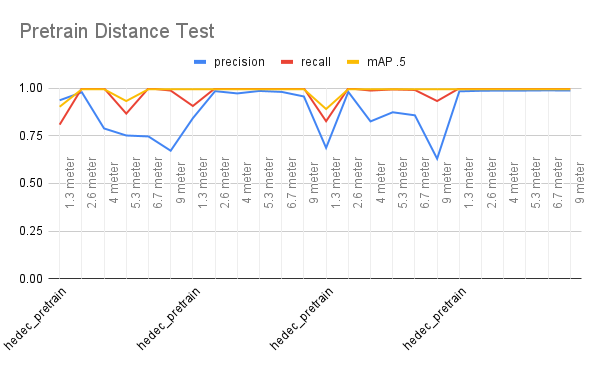
\includegraphics[width=0.4\textwidth]{gambar/utilities/pretain_dist_test.png}
  \caption{Pretrained Model Distance Difference Test}
  \label{fig:pretrain_dist_test}  
\end{figure}

\begin{figure}[ht]
  \centering
  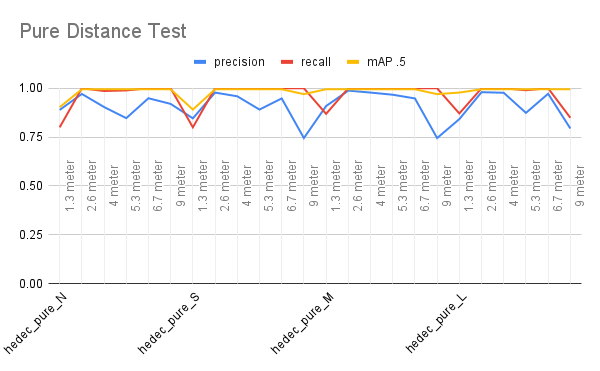
\includegraphics[width=0.4\textwidth]{gambar/utilities/pure_dist_test.png}
  \caption{Without Pretrained Model Distance Difference Test}
  \label{fig:pure_dist_test}  
\end{figure}

\subsection{Model Performance Benchmark on Low Illuminance}
\label{subsec:model_lowillum_test}

\par This section describes the model's performance in detecting low-brightness input images. The validation data contains 35 images with the number of labels no\textunderscore helmet 20 and labels with\textunderscore helmet 57. In addition, validation is carried out on the training results using pre-trained weight and those without pre-trained weight. The test conducted using all the available weight variants as show in Figure~\ref{fig:lowillum_test}.

\begin{figure}[ht]
  \centering
  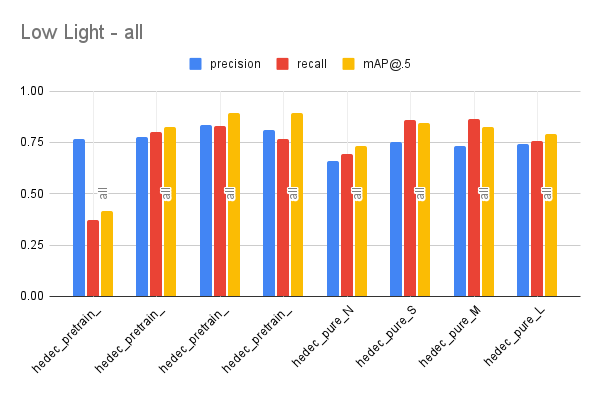
\includegraphics[width=0.4\textwidth]{gambar/utilities/lowlight_test.png}
  \caption{Low Illuminance Test}
  \label{fig:lowillum_test}  
\end{figure}

\subsection{Frame Rate Test on Jetson Nano}
\label{subsec:model_jetsonnano_test}

\par This section is an explanation of the results of the YOLOv5 Model performance testing when being run on Jetson Nano with the weights that have been previously trained Nano. This test aims to compare the effectiveness of each weight that has been made on the inference performance aspect, considering that the Jetson Nano is a mini-computer with its own Graphics Processing Unit (GPU) and is designed for AI IoT applications. Therefore, the measurement taken in this test is the Frame Per Second (FPS) value.

 
\par Tests were carried out using the Nemesis NYK A-90 Everest Webcam attached to the Jetson Nano via a USB cable. The tests were carried out at resolutions 256, 480, and 640. The results of the FPS measurement on the YOLOv5 Helmet Detection test are presented in Table~\ref{tb:jetsonano_model_benchmark}.

\begin{table}
  \centering
  \caption{Jetson Nano Model Framerate Benchmark}
  \label{tb:jetsonano_model_benchmark}
  \begin{tabular}{|l|l|l|l|} 
    \hline
    \multirow{2}{*}{\textbf{Nama Bobot}} & \multicolumn{3}{l|}{\textbf{Resolusi}}      \\ 
    \cline{2-4}
                                         & \textbf{256} & \textbf{480} & \textbf{640}  \\ 
    \hline
    hedec\_pretrain\_N                   & 24.4         & 22           & 18.5          \\
    hedec\_pretrain\_S                   & 22.2         & 13           & 7.8           \\
    hedec\_pretrain\_M                   & 15.2         & 5.7          & 3.4           \\
    hedec\_pretrain\_L                   & 8            & 3.2          & 1.8           \\
    hedec\_pure\_N                       & 24.9         & 21.5         & 18.4          \\
    hedec\_pure\_S                       & 23           & 12.3         & 7.8           \\
    hedec\_pure\_M                       & 15           & 5.4          & 3.3           \\
    hedec\_pure\_L                       & 8.3          & 3            & 1.8           \\
    \hline
  \end{tabular}
\end{table}


\subsection{Hardhat Detection System Field Test}
\label{subsec:hedect_sys_test}

\par This subsection will display various tests on the helmet detection system. The workflow of the Hardhat Detection System is previously explained in Subsec~\ref{subsec:hedect_dev_sys} as also explained on there that the system will trigger an alarm in the form of a siren alarm when there is one or more "no\_helmet" class is detected within the frame. 

\par The tests mostly are done by taking samples of frames from recorded system testing on various conditions: distance difference, low illuminance, CCTV angle, and Jetson Nano run. For this test, as it focuses on "How accurately the system fired the alarm when actually needed to", the "positive" is seen from when the alarm is triggered, and the "negative" are seen from when the alarm is not activated. The variant of weight used in these test is "hedec\_pretrain\_S".

\subsubsection{System Test on Distance Difference}
\label{subsubsec:hedect_test_dist}

\par This test is conducted with the various distance between the camera and the object (person wearing and not wearing a hardhat) observed. The test is conducted by taking samples of frames from a predicted pre-recorded video with a person moving and rotating from 1 meter to 10 meters. The result of each distance variants are shown in Table~\ref{tb:systest_dist_test}.

\begin{table}
  \centering
  \caption{System Test on Distance Difference}
  \label{tb:systest_dist_test}
  \begin{tabular}{|l|l|l|l|l|l|l|} 
  \hline
  Distance & TP & TN & FP & FN & Accuracy     & Samples of Test  \\ 
  \hline
  1m       & 17 & 61 & 7  & 0  & 0.9176470588 & 85               \\ 
  \hline
  3m       & 20 & 44 & 0  & 2  & 0.9696969697 & 66               \\ 
  \hline
  5m       & 40 & 53 & 0  & 0  & 1            & 93               \\ 
  \hline
  7m       & 32 & 56 & 0  & 0  & 1            & 88               \\ 
  \hline
  10m      & 78 & 32 & 0  & 0  & 1            & 110              \\
  \hline
  \end{tabular}
\end{table}


\subsubsection{System Test on CCTV angle}
\label{subsubsec:hedect_test_cctv}

\par This test is conducted to imitate how CCTV is placed at a checkpoint on a construction site which usually is at a 45-degree angle. The test results are showin in Table~\ref{tb:systest_cctv}.

\begin{table}
  \centering
  \caption{System Test on CCTV angle}
  \label{tb:systest_cctv}
  \begin{tabular}{|l|l|l|l|l|} 
  \hline
  TP & TN & FP & FN & Accuracy         \\ 
  \hline
  27 & 28 & 0  & 9  & 0.859375         \\ 
  \hline
  \multicolumn{2}{|l|}{55}   & \multicolumn{2}{l|}{9} & 64 test samples  \\
  \hline
  \end{tabular}
\end{table}


\subsubsection{Realtime Detection Test in Jetson Nano}
\label{subsubsec:hedect_test_cctv_jetsonanno}

\par This test is also conducted to imitate how CCTV is placed at a checkpoint on a construction site, usually at a 45-degree angle. But the difference is that the system is being run in real-time. Unlike the other test where the prediction is being done on a pre-recorded video, in this test, the prediction is being run in real-time as the system actively detects using the webcam feeds. The test results are shown in Table~\ref{tb:systest_jetsonnano}.

\begin{table}
  \centering
  \caption{Realtime Detection Test in Jetson Nano}
  \label{tb:systest_jetsonnano}
  \begin{tabular}{|l|l|l|l|l|} 
  \hline
  TP & TN                    & FP & FN                & Accuracy         \\ 
  \hline
  14 & 17                    & 0  & 2                 & 0.9393939394     \\ 
  \hline
  \multicolumn{2}{|l|}{31}   & \multicolumn{2}{l|}{2} & 33 test samples  \\
  \hline
  \end{tabular}
\end{table}

\subsubsection{System Test in Low Illuminance (Dusk)}
\label{subsubsec:hedect_test_lowillum_dusk}

\par This test is also conducted at a dusk time when illuminance is fairly low, and the sky is still lit. The test result is shown on Table~\ref{tb:systest_lowillum_dusk}. For this test there is 75 samples of test.

\begin{table}
  \centering
  \caption{System Test in Low Illuminance (Dusk)}
  \label{tb:systest_lowillum_dusk}
  \begin{tabular}{|l|l|l|l|l|} 
  \hline
  TP & TN                    & FP & FN                & accuracy         \\ 
  \hline
  45 & 25                    & 0  & 5                 & 0.9333333333    \\ 
  \hline
  \multicolumn{2}{|l|}{31}   & \multicolumn{2}{l|}{2} & 33 test samples  \\
  \hline
  \end{tabular}
\end{table}

\subsubsection{System Test in Low Illuminance (Dark)}
\label{subsubsec:hedect_test_lowillum_dark}

\par This test is also conducted at a dusk time when illuminance is very low with only one light source. The test result is shown on Table~\ref{tb:systest_lowillum_dark}. For this test there is 250 samples of test.

\begin{table}
  \centering
  \caption{System Test in Low Illuminance (Dark)}
  \label{tb:systest_lowillum_dark}
  \begin{tabular}{|l|l|l|l|l|} 
    \hline
    TP & TN                     & FP & FN                 & Accuracy  \\ 
    \hline
    40 & 139                    & 0  & 71                 & 0.716     \\ 
    \hline
    \multicolumn{2}{|l|}{179}   & \multicolumn{2}{l|}{71} &           \\
    \hline
  \end{tabular}
\end{table}

